% !TEX root = ../AGAO.tex

\section{The Cut-Matching Game: Expanders via Max Flow}


We define the expanders and similar things here, that may be different than in the chapter $7$.

\begin{definicija}
    Let $G$ be an unweighted, connected graph here and $\dd$ be the degree vector. $E(S , V\setminus S)$ denotes the edges crossing the cut between $S$ and $V\setminus S$.

    The \textit{sparsity} $\psi(S)$ of the cut is defined by 

    \begin{align*}
        \psi (S) = \frac{\mid E ( S, V\setminus S) \mid}{\min ( |S|, |V \setminus S| )}
    \end{align*}
    So we look at the edges divided by the min vertices in the left or right side.

    
    Remember, that sparsity is different than conductance, which was defined by dividing the edges with the min volume, which is the number of edges that have atleast one end in this set.

    So the \textit{conductance} is defined as

    \begin{align*}
        \phi(S) = \frac{\mid E ( S, V\setminus S) \mid}{\min ( vol|S|, vol|V \setminus S| )}
    \end{align*}


    And similar as for conductance the \textit{sparsity} of the graph $G$ is $\min _S\psi (S)$.

    We also see that in a connected graph we have $\psi(S) \geq \phi(S)$, because if there is no edge in the cut  we are done and if there is, then the volume is at least the size of the set, because we are connected.

    For any $\psi \in (0, n]$ we say that $G$ is a $\psi$ expander if $\psi(G) \geq \psi$.

    Here we could say it is expander with regard to sparsity, but we will just say it is an expander if it is obvious we mean sparsity.
\end{definicija}


So we have a main theorem here, that we have some kind of good algorithm

\begin{izrek}
    There is an algo \texttt{SPARSITY CERTIFY OR CUT} that given a graph $G$, and parameter $0 < \psi \leq 1$ that either:

    \begin{itemize}
        \item Certifies that $G$ is an $\Omega (\psi / \ln ^2 n)$ - expander with regard to sparsity or

        \item Presents a cut $S$ such that $\psi(S) \leq O(\psi)$
    \end{itemize}
    The algo runs in time $O(\ln ^2 n) \cdot T_{max flow}(G) + \Tilde{O}(m),$
    where $T_{max flow}(G)$ is the time it takes to solve Max Flow problem on $G$ (with two additional vertices and $n$ edges, but this doesn't change the runtime).
\end{izrek}

Apparently, we can use the bounds above to also compute conductance expanders. And using state of art Max Flows we can solve this all in $O(m^{1 + o(1)}).$

I have no idea how it should work, but oh well.

\subsection{Embedding Graphs into Expanders}

\begin{definicija}
    Given graphs $H, G$ with same vertex set, we say that a function \texttt{EMBED}$_{H \rightarrow G}$ is an \textit{embedding} if it maps each edge $(u,v) \in H$ to a $u-v$ path $P_{u,v} = $ \texttt{EMBED}$_{H \rightarrow G}(u,v)$ in $G$.
\end{definicija}

\begin{figure}[h]
\centering
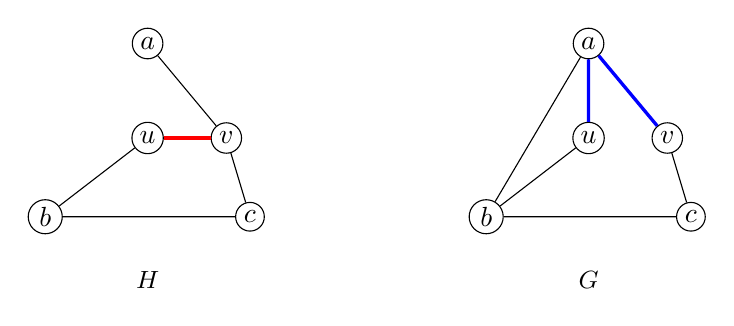
\begin{tikzpicture}[
  scale=1.0,
  vtx/.style={circle,draw,inner sep=1.5pt},
]
  % Left: H
  \begin{scope}[xshift=0cm]
    \node[vtx] (Hu) at (1,1) {$u$};
    \node[vtx] (Hv) at (2,1) {$v$};
    \node[vtx] (Ha) at (1,2.2) {$a$};
    \node[vtx] (Hb) at (-0.3,0) {$b$};
    \node[vtx] (Hc) at (2.3,0) {$c$};

    \draw (Ha) -- (Hv) -- (Hc) -- (Hb) -- (Hu);
    

    % highlight an edge (u,v) in H
    \draw[very thick,red] (Hu) -- (Hv);

    \node[font=\small] at (1,-0.8) {$H$};
  \end{scope}

  % Right: G
  \begin{scope}[xshift=5.6cm]
    \node[vtx] (Gu) at (1,1) {$u$};
    \node[vtx] (Gv) at (2,1) {$v$};
    \node[vtx] (Ga) at (1,2.2) {$a$};
    \node[vtx] (Gb) at (-0.3,0) {$b$};
    \node[vtx] (Gc) at (2.3,0) {$c$};

    \draw (Gu) -- (Gb) -- (Gc) -- (Gv);
    \draw (Gb) -- (Ga) -- (Gv);
    \draw (Gu) -- (Ga);

    % highlight a u-v path in G as the image of (u,v)
    \draw[very thick,blue] (Gu) -- (Ga) -- (Gv);

    \node[font=\small] at (1,-0.8) {$G$};
  \end{scope}
\end{tikzpicture}
\caption{An example of an embedding: the edge $(u,v) \in H$ (red) is mapped to the $u$--$v$ path $u-a-v$ in $G$ (blue).}
\end{figure}

\begin{definicija}
    We say that the \textit{congestion} of the embed is the maximum  umber of times that any edge $e \in E(G)$ appears on any embedding path.

    \begin{align*}
        cong(\texttt{EMBED}_{H \rightarrow G}) = \max _{e \in E(G)}|\{e' \in E(H) | e \in \texttt{EMBED}_{H \rightarrow G(e)}\}|
    \end{align*}
\end{definicija}

Now we get to a lemma that connects the embedding with the expanders.

\begin{lema}
    Given a $\frac 1 2$ expander $H$ and an embedding $H$ into $G$ with congestion $C$, then $G$ must be an $\Omega (\frac 1 C )$ expander.
\end{lema}

\begin{proof}
    Take any cut $S$ smaller than half of the vertices. Since $H$ is an expander we know that $|E_H ( S, V \setminus S)| \geq |S|/2$. For each edge that crosses from $S$ we also know that it has to cross into that in the embedding at least once. But each edge is traversed at most $C$ times, so we have that at least $|S|/2C$ edges in $G$ cross the cut.
\end{proof}

The reverse doesn't hold. Why do I need this? I am not sure yet tbh.

\subsection{The Cut-Matching algorithm}

Now lets directly discuss the algorithm and see why and how it works.


\begin{algorithm}
\caption{SPARSITYCERTIFYORCUT}\label{alg:sparsitycertifycut}
\begin{algorithmic}
\For {$i = 1, 2, \ldots, T$} \\
\State $(S_i, \overline{S_i}) \gets \texttt{FIND BI PARTITION}(G, \{M_1, \ldots, M_i\});$
\Comment{Assume $S$ has exactly half vertices.}\\
\State Solve the flow problem on $G$ where each edge $e$ receives same capacity $\ccc (e) = 1/\psi $ and the demand at each vertex in $S$ is $1$ and $-1$ in the complement. We can do this by introducing the super sources $s$ with demand $n/2$ and is connected to every element in $S$ and each edge from $S$ carries exactly one capacity. Similar for the sink $t$.
\\
\If{we get a flow with $val(f) = n/2$}
    \State Remove $s,t$ to get $S-\overline{S}$ flow, then decompose flow $f$ into flow paths $P_1, \ldots, P_{n/2}$
    \State Create Matching $M_i$, where for each flow path $P_i$ we add the starting and ending vertex as a virtual edge
\Else
    \State Let $(X \cup s, \overline{S} \cup t)$be the $st$ min cut in the flow problem.
    \State Return $(X, \overline{X})$
\EndIf
\EndFor
\State \Return $\cup _i M_i$
\end{algorithmic}
\end{algorithm}


We will later see that $T$ is $O(\ln ^2 n)$.

So how does this actually work. We take the bipartition and we use it to find the flow problem. We will actually define the \texttt{FIND BIPARTITION} later so we know which one to choose.

But in each iteration we first get the partition, which makes a cut of equal sizes. Next we create a flow problem that reminds us a lot of the sparsity expander thing. We create the flow with introducing the super source and super sink and this essentially means that we want to transfer $1$ from each vertex on the left to each vertex on the right. And we set the capacity of edges in the original graph to be $1/\psi$, which for some reason they say is wlog integer, but I dont trust them tbh.

If we can solve the whole flow, that means that we can decompose the flow into paths (using DFS for example) so that each path starts in $S$ and ends in complement. This gets us the matching $M_i$.

We will see that if we combine all the matchings into a graph $H$ while using $ T = \Theta(\ln ^2 n)$ matchings then we should get that the graph $H$  is a $1/2$ expander and can be embedded into $G$ with congestion $O(\ln^2 n / \psi)$. I honestly have no idea where this comes from, it is a lemma from the script, but seems kinda weird I think. But from this and the previous lemma we can get that $G$ is an appropriate expander (so we certify that).

Now if we cant solve that, then we return the min cut of the flow problem, which can be done efficiently once we have the maximum flow. Should be in $O(m)$ time they say.

And now that min cut should have sparsity of $O(\psi)$ by the way it was defined.

\begin{lema}
    If algo terminates with a cut $X, \overline{X}$, then $\psi (X) = O(\psi)$.
\end{lema}


\begin{proof}
    We add $s,t$ back to the sets and observe that since the whole flow didnt make it to $t$, we have in this cut less than $n/2$ capacity (because it is min cut). Now we look at the edges that cross the cut, they might be original or new from $s, t$. Let $n_s$ be the number of edges from $s$ crossing the cut and similarly $n_t$. Each of those edge routes $1$ and other edges route $1/\psi$. After we take away the vertices $s,t$ we are routing less than $n/2 - n_s - n_t$. So the total number of original edges crossing is atmost $\psi (n/2 - n_s -n_t)$

    Now we can calculate that $X$ is of size atleast $n/2 - n_s$, because $s$ has degree $n/2$ and exactly $n_s$ edges go to the other side.

    Similarly for $\overline{X}$.

    So we have 

    \begin{align*}
        \psi(X) < \frac{\psi ( n/2 - n_s - n_t)}{\min(n/2 - n_s, n/2 - n_t)} \leq \psi
    \end{align*}
\end{proof}

And thats a pretty cool proof, you gotta remember all the bounds we used before.


Remember, we now still have to prove that $H$ will be a $1/2$ expander, that $T$ will be of the form we want and that all the $O$s in the if part are ok. And we gotta define the bipartition.


\subsection{Bipartition with random walks}

We start from some random walks on matchings.

\begin{definicija}
    Suppose we have a set of matchings $M_1, \ldots, M_T$ that we computed (we never found a cut). In the $i$-th step of the lazy random walk we let the mass at each vertex stay put with probability $1/2$ and to traverse to the matching neighbour in $M_i$ with $1/2$.

    Now we denote with $p_{j \rightarrow i} ^t$ the probability that a particle that started at vertex $j$ is at vertex $i$ after a $t$-step lazy random walk.

    And $\mathbf{p}_i^t = [p_{1 \rightarrow i}^t, \ldots, p_{n \rightarrow i}^t]^\top$

    Obviously we have that if $i,j$ is an edge in $M_{i+1}$ then $\mathbf{p}_i^{t+1} = \mathbf{p}_i^{t}/2 + \mathbf{p}_j^{t}/2 = \mathbf{p}_j^{t+1}$.

    Now we can combine all those probabilities to a matrix $\Pi^t =[\mathbf{p}_i^{t}]^\top$. This matrix maps the initial distribution to the distribution after $t$ steps.

    If the lazy walk gets approximately uniform we will say it is mixing

    \begin{definicija}
        We say a lazy random walk is \textit{mixing} at step $t$ if all $p_{j \rightarrow i} ^t \geq \frac{1}{2n}$
    \end{definicija}

    \begin{lema}
        If $t$ step lazy random walk is mixing, then $H = \cup M_{i\leq t}$ is a $\frac 1 2$ expander
    \end{lema}

    \begin{proof}
        Take any cut that has less than half of the vertices. We can think of the walk as moving mass around. So we need each vertex to move atleast $1/2n$ mass to travel between any two vertices.

        We can say that we are moving from $\overline{S}$ to $S$. So then each vertex in the complement needs to push mass over the edges in matchings that cross the cut. 

        But since the complement has at least half of the vertices, the total mass pushed over has to be at least $1/4$ for each $i$. So in total $\geq |S|/4$ mass must cross the cut. But at each step, each edge in $M_i$ can transfer at most $1/2$ units and then it gets deleted and replaced with next matching edges.

        So it follows that in matchings $M_1, \ldots, M_t$ there appear atleast $|S|/2$ edges crossing the cut, so $H$ must be a $1/2$ expander.
    \end{proof}


    We now provide implementation for \texttt{FIND BIPARTITION} and we explain it later.

    \begin{algorithm}
    \caption{FIND BIPARTITION($G, M_1, \ldots, M_t$)}\label{alg:findbiparition}
    \begin{algorithmic}

    \State Choose random $n$ dimensional vector $\mathbf{r} \perp \mathbf{1}$.
    \State Compute the distribution after $t$ steps as if we start from $\mathbf{r}$ distribution (honestly, it is not a valid distribution, but who cares). Then $\mathbf{u} = \Pi ^t \mathbf{r}$
    \State Let $S$ be the $n/2$ smallest vertices in $\mathbf{u}$ and in the complement we take the largest (ties arbitrarily, but consistently)
    \State \Return $(S, \overline{S})$
    \end{algorithmic}
    \end{algorithm}

    This algo looks very random, but what can I do? It might make sense in some way but currently it doesn't make any sense, hurrayyy.


    Now we will introduce a potential function

    \begin{align*}
        \Phi ^t = \sum_{ij} (p_{i \rightarrow j}^t - 1/n )^2 = \sum_i \| \mathbf{p}_i ^t - \mathbf{1}/n \|_2 ^2
    \end{align*}

    Man the proof of this is too complicated for today, hopefully I revisit it next time, glhf.

    
    

    
    
\end{definicija}